
\begin{itemize}
\item{\textbf{Kratak opis:} Administrator unosi informacije o klijentu koji u trenutku unosa ne postoji u sistemu. Sistem obradjuje informacije, az1urira se stanje sistema i vrac1a povratna informacija o uspeshnosti unosa.}
\item{\textbf{Akteri:} Administrator sistema}
\item{\textbf{Ulaz:} Podaci o klijentu }
\item{\textbf{Izlaz:} Poruka o uspeshnosti unoshenja klijenta u sistem }
\item{\textbf{Preduslovi:} Administrator ima pristup sistemu i poseduje potrebne informacije o novom klijentu. Postoji komunikacija izmedju administratora i klijenta. }
\item{\textbf{Postuslovi:} Uspeshno dodat klijent u sistem.}
\item{\textbf{Glavni tok:} Administrator unosi traz1ene podatke o novom klijentu (naziv kompanije, PIB i MB kompanije, sedishte, broj aktivnih magacina, adrese aktivnih magacina). Sistem validira podatke i az1urira stanje. Nakon toga prikazuje se potvrda o uspeshnosti akcije. }
\item{\textbf{Alternativni tokovi:} Neuspeshno dodavanje klijenta.}
\end{itemize}
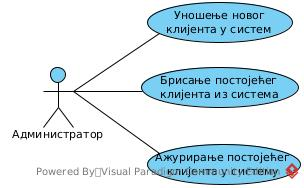
\includegraphics{Slike/SUadministrativniPoslovi.jpg}